%\PassOptionsToPackage{style=apa,backend=biber,doi=true,natbib=true,url=true}{biblatex}
\documentclass[floatsintext,a4paper]{apa7} %man,mask
\usepackage[utf8]{inputenc}
\usepackage[style=apa,backend=biber,doi=true,natbib=true,url=true]{biblatex}
\addbibresource{SEMmisfit.bib}
\usepackage{amsmath} %for multiple line equations
\usepackage{graphicx}
%\usepackage{blkarray}
\usepackage{cuted}
%\usepackage{comment}
%\usepackage{appendix}

\usepackage{booktabs}      % for \toprule, \midrule, \bottomrule
% \usepackage{longtable}     % if longtable output is used
\usepackage{array}         % for >{} column specifiers and \arraybackslash
% \usepackage{multirow}      % if multirow features are used
\usepackage[table]{xcolor} % for \cellcolor and alternating row colors
\usepackage{colortbl}      % color support in tables

\makeatletter
\providecommand{\@setmarks}{}
\makeatother



%% for external document (eg appendix) reference linking
%\usepackage{xr}
%\makeatletter
%\newcommand*{\addFileDependency}[1]{% argument=file name and extension
	%	\typeout{(#1)}
	%	\@addtofilelist{#1}
	%	\IfFileExists{#1}{}{\typeout{No file #1.}}
	%}
%\makeatother
%
%\newcommand*{\myexternaldocument}[1]{%
	%	\externaldocument{#1}%
	%	\addFileDependency{#1.tex}%
	%	\addFileDependency{#1.aux}%
	%}
%
%\myexternaldocument{supplement}

\usepackage{bm} 
\newcommand{\vect}[1]{\boldsymbol{\mathbf{#1}}}

\title{Residual Diagnostics for SEM Misfit Beyond Mean and Covariance Fit}

\shorttitle{Residual Diagnostics for SEM Misfit}
\authorsnames{{Charles C. Driver},{Others}}
\authorsaffiliations{{University of Zurich, Switzerland}}

\authornote{
	Analyses were not preregistered. Scripts to reproduce the simulation, empirical example, generated figures, and prototype diagnostic workflow are available in the online supplementary material. Correspondence concerning this article should be addressed to Charles C. Driver, Department of Psychology, University of Zurich, Binzm\"uhlestrasse 14, Box 28, 8057 Zurich, Switzerland. E-mail: charles.driver@psychologie.uzh.ch
}
\leftheader{Driver}


\abstract{
	Structural Equation Modeling (SEM) remains a cornerstone of psychological research, providing a means of testing complex theoretical models. Classical SEM fit indices are useful diagnostics for their usual target: whether a fitted model reproduces the observed mean vector and covariance matrix sufficiently well. However, covariance and mean fit do not exhaust the kinds of structure that can matter in psychological data. Nonlinear residual dependence, subgroup heterogeneity, heavy tails, outliers, and marginal nonnormality can remain after a model fits first- and second-order moments. We therefore frame residual diagnostics as a decomposition of model-checking targets rather than as a replacement for classical SEM fit. The proposed workflow separates baseline covariance/mean fit, residual distribution checks, residual-dependence checks, and localization tools for variables, pairs, and cases. This distinction is important because broad distributional tests can flag many departures from the fitted Gaussian reference, whereas independence tests such as distance covariance or dHSIC more directly target residual dependence after whitening. Simulations and software are used to illustrate how these diagnostics can complement standard SEM output and guide follow-up modeling without treating every normality violation as substantive SEM misspecification.
}    


\keywords{structural equation model, SEM, model fit, misspecification, nonlinear}

\begin{document}
	\maketitle
	
	\section{Introduction}
	Structural Equation Modeling (SEM) has long been a foundational tool in psychological research, enabling scholars to test complex theoretical models that encompass multiple interrelated constructs \citep{bollen1989structural}. Central to SEM's utility is the ability to assess model fit, which determines how well a proposed model aligns with the observed data. Global misfit tests, such as the chi-square test of model fit, Comparative Fit Index (CFI,\cite{bentler1990comparative}), Tucker-Lewis Index (TLI,\cite{hu1999cutoff}), Root Mean Square Error of Approximation (RMSEA), and Standardized Root Mean Square Residual (SRMR), are commonly employed to evaluate this alignment.
	
	A global test of model misfit is, conceptually, extremely appealing, as it enables a researcher to easily determine whether their specified model provides a reasonable representation of the data, thereby raising confidence in any inferences that result from the model. As usual however, implementation details and assumptions are critical. Standard SEM fit tests and indices primarily assess discrepancies between the observed and model-implied means and covariance matrix. That target is valuable: many SEM hypotheses are expressed as restrictions on means, variances, covariances, factor loadings, and regression paths. At the same time, psychological data can also exhibit \textbf{complex dependencies, subgroup heterogeneities, and nonlinear interactions} \citep{micceri1989unicorn} that do not necessarily produce large residuals in the covariance matrix. A model may therefore fit the classical moment target while still leaving structured residual dependence or distributional departures that are scientifically relevant.
	
	To address these limitations, we examine \textbf{residual-based diagnostics} that complement standard SEM fit output. The goal is diagnostic decomposition: different checks should be interpreted according to the residual null they target. The novelty is not the invention of each component test, but the integration of existing SEM fit, residual-distance, distributional, and nonparametric independence-testing tools into a single workflow for fitted SEM residuals. This integration is timely because recent SEM work has continued to develop nonlinear latent-interaction methods, nonlinear SEM power tools, robust fit-index handling under nonnormal and missing data, Bayesian fit indices, and tree/forest approaches for heterogeneity and specification search \citep{irmer2024estimating,cox2025comparing,jia2026obtaining,garnierVillarreal2020adapting,arnold2021score,silvaDiaz2025evaluation}. In the current work we distinguish:
	
	\begin{enumerate}
		\item \textbf{baseline SEM moment fit}, which assesses mean and covariance reproduction;
		\item \textbf{residual distribution checks}, including multivariate normal energy tests \citep{rizzo2016energy} and classical AD / KS / CVM style checks against expected residual distributions;
		\item \textbf{residual-dependence checks}, including distance covariance and dHSIC (Hilbert-Schmidt Independence Criterion) in bivariate and multivariate contexts \citep{pfister2018kernelbased}; and
		\item \textbf{localization diagnostics}, including variable-level, pairwise, and case-level residual summaries that guide follow-up modeling.
	\end{enumerate}
	
	This decomposition avoids treating all normality violations as evidence for the same kind of model failure. A marginal residual normality test may flag skewness, heavy tails, or outliers without indicating residual dependence among variables. A multivariate residual distribution test can be sensitive to many forms of departure from the fitted Gaussian reference, including mixtures and tail behavior. A residual-dependence test asks a narrower question: whether residual coordinates remain dependent after whitening by the model-implied covariance. That narrower target is especially relevant when the substantive concern is an omitted nonlinear association or interaction.
	
	While traditional SEM software packages are optimized for moment-structured models, emerging methodologies offer avenues to model structure discovered through residual diagnostics. Approaches such as incorporating covariate moderators, specifying interactions, using flexible parametric terms, employing Bayesian estimation techniques, mixture or latent-class models, and utilizing tree- or forest-based SEM models can accommodate some nonlinearities and subgroup heterogeneities \citep{mcdonald1962general,klein2000maximum,irmer2024estimating,cox2025comparing,lubke2005investigating,brandmaier2013structural,briley2015nonparametric,arnold2021score,silvaDiaz2025evaluation,muthen2012bayesian,garnierVillarreal2020adapting}. Residual diagnostics do not by themselves identify the correct revision, but they can indicate which aspect of fit has failed and where follow-up modeling should begin.
	
	In the following sections we first briefly outline the typical SEM modeling approach and model fit testing approach. We then describe residual representations and diagnostic targets, separating checks of mean/covariance fit, residual distributions, residual dependence, and localization. We then simulate data under various misfit conditions and compare performance between classical SEM chi-square tests and a variety of residual-based diagnostics. We then discuss approaches that can be taken when residual diagnostics suggest nonlinear dependence or other structured departures -- how can one go about finding exactly where the misspecification lies, and what modeling approaches could be considered. We finish with proposed guidelines, pointers to relevant approaches and software, and discussion of what is still needed.
	
	\section{SEM \& Model Fit}
	
	Structural Equation Modeling (SEM) is a statistical technique that integrates elements of factor analysis and multiple regression to evaluate complex theoretical models involving multiple interrelated constructs. SEM allows researchers to specify and test models that encompass both measurement components (i.e., how latent constructs are measured by observed indicators) and structural components (i.e., the hypothesized relationships among latent constructs).
	
	The SEM approach typically begins with the specification of a theoretical model, which delineates the hypothesized relationships among latent variables and their corresponding observed indicators. This model usually comprises two parts: the measurement model and the structural model. The measurement model defines how latent constructs are operationalized through observed variables, while the structural model specifies the directional relationships among these latent constructs.
	
	Parameter estimation in SEM is commonly performed using Maximum Likelihood (ML) estimation, which seeks to find the parameter values that maximize the likelihood of observing the given data under the specified model. Other estimation methods, such as Generalized Least Squares (GLS) and Bayesian estimation, are also employed depending on the nature of the data and the specific requirements of the analysis, however for the purposes of this work we will focus on continuous data and typical SEM modeling practices.
	
	\subsection{Assessing Model Fit}
	
	A critical aspect of SEM is the evaluation of how well the proposed model fits the observed data. Global model fit indices are employed to provide an overall assessment of model adequacy by comparing the covariance structure implied by the model to the empirical covariance matrix derived from the data. Commonly used fit indices include:
	
	\begin{itemize}
		\item \textbf{Chi-square Test of Model Fit}: Calculates the probability of observing the difference in likelihood between the proposed model fit and a saturated model fit, under the assumption that the proposed model provides an adequate representation of the data. A non-significant chi-square value ($\chi^2$) indicates good model fit, suggesting that the model-implied covariance matrix does not significantly differ from the observed covariance matrix.
		
		\item \textbf{Comparative Fit Index (CFI)}: Compares the fit of the proposed model to that of a baseline model, typically the null model which assumes no relationships among variables. The CFI assesses the improvement in fit of the proposed model over the baseline by taking into account the degrees of freedom and sample size. It ranges from 0 to 1, with values closer to 1 indicating better fit. Values above 0.95 are generally indicative of good fit, reflecting a substantial improvement over the baseline model.
		
		\item \textbf{Tucker-Lewis Index (TLI)}: Similar to the CFI, the TLI compares the fit of the proposed model to a baseline model but incorporates a penalty for model complexity. The TLI adjusts for the number of parameters estimated in the model, thereby discouraging overly complex models that do not provide significant improvement in fit. Values above 0.95 suggest adequate fit, indicating that the proposed model achieves a good balance between fit and parsimony.
		
		\item \textbf{Root Mean Square Error of Approximation (RMSEA)}: Measures the lack of fit per degree of freedom in the proposed model. The RMSEA evaluates how well the model, with optimally chosen parameter estimates, would fit the population covariance matrix. It accounts for model complexity by penalizing models with more parameters, providing a parsimonious measure of fit. Values below 0.06 are considered indicative of good fit, with lower values representing better fit.
		
		\item \textbf{Standardized Root Mean Square Residual (SRMR)}: Represents the standardized difference between observed and predicted correlations. The SRMR quantifies the average discrepancy between the observed covariance matrix and the model-implied covariance matrix, standardized by the variance of the observed variables. Values below 0.08 are typically deemed acceptable, indicating that the model's predictions closely align with the observed data.
	\end{itemize}
	
	These fit indices provide complementary information about model adequacy, allowing researchers to make informed judgments about the validity of their theoretical models. Their primary target is mean and covariance reproduction, often under a likelihood framework that uses a multivariate normal reference for continuous data. Robust corrections, bootstrap procedures, and recent work on robust practical fit indices address some consequences of nonnormality, missingness, and imputation for SEM test statistics and fit summaries \citep{satorra1994corrections,bollen1992bootstrapping,jia2026obtaining}, but they do not turn global moment-fit indices into diagnostics for every residual feature of the observed data distribution.
	
	\subsection{Implications for Theory Testing and Model Development}
	
	The target of traditional SEM fit indices has significant implications for theory testing and model development in psychology. When theories imply nonlinear associations, interactions, subgroup-specific relations, or residual heterogeneity, a covariance-based fit summary may be incomplete even when it is correctly computed and useful for its intended purpose. This limits the scope for incremental model building if researchers treat acceptable global moment fit as evidence that no further structure remains.
	
	Moreover, unmodeled complex data phenomena can lead to incomplete inferences about model adequacy, potentially resulting in the acceptance of models that fit means and covariances but miss substantively important higher-order structure. The field therefore needs practical residual diagnostics that can be applied alongside classical SEM output, with clear labels for what each diagnostic tests and what it does not test.
	
	\section{Residuals in SEM}
	
	Residuals in Structural Equation Modeling (SEM) provide essential diagnostic information about model misfit. Different conceptualizations of residuals allow for varying levels of specificity in detecting model deficiencies, ranging from global deviations in implied covariance structures to fine-grained, observation-level discrepancies. Below, we outline four primary types of residuals in SEM, each offering distinct advantages for assessing different aspects of model fit.
	
	\subsection{Residuals of the Expected vs. Implied Covariance Matrix}
	The most traditional residuals in SEM are computed as the difference between the \textbf{empirical (observed) covariance matrix} $ S $ and the \textbf{model-implied covariance matrix} $ \Sigma(\theta) $:
	
	$$
	R_{\Sigma} = S - \Sigma(\theta).
	$$
	
	This residual matrix captures a central component of \textbf{global model fit}, assessing how well the specified model reproduces the \textbf{second-order (covariance) structure} of the data. If the residuals in $ R_{\Sigma} $ are large, it suggests that the model fails to account for the observed linear relationships between variables. However, this residual matrix is limited to the moment target it represents. It does not directly test \textbf{nonlinear dependencies, heteroscedasticity, subgroup structure, or individual-level deviations} unless these departures also affect the fitted means or covariance matrix.
	
	\subsection{Unstandardized Raw Data Residuals}
	At the level of individual observations, raw residuals are computed as the deviation of each observation from the model-implied \textbf{mean vector} $ \mu(\theta) $:
	
	$$
	R_{\text{raw},i} = X_i - \mu(\theta),
	$$
	
	where $ X_i $ is the vector of observed variables for individual $ i $. These residuals are useful in detecting \textbf{mean structure misfit}, outliers, and \textbf{patterned deviations} in the data. However, unstandardized residuals may not be directly comparable across variables due to differences in measurement scales.
	
\subsection{Standardized Residuals via Symmetric Whitening}
To make raw residuals comparable across dimensions, the prototype standardizes (or ``whitens'') them using the \textbf{symmetric inverse square root} of the model-implied covariance matrix:
	
	$$
R_{\text{ZCA}, i} = (X_i - \mu(\theta))\Sigma(\theta)^{-1/2},
	$$
	
where $\Sigma(\theta)^{-1/2}$ is the symmetric inverse square root of $\Sigma(\theta)$. This transformation ensures that, under the fitted Gaussian observed-data model, the standardized residuals should follow a standard multivariate normal distribution, with \textbf{mean zero and identity covariance}:
	
	$$
R_{\text{ZCA}, i} \sim \mathcal{N}(0, I).
	$$
	
Symmetric whitening is equivariant to a common reordering of the observed variables and covariance matrix. Its coordinates are nevertheless transformed coordinates, not original-variable residuals. The prototype retains Cholesky innovations only as an explicitly order-dependent comparison representation; it does not use them for global tests or variable-labelled pairwise output. If the fitted Gaussian observed-data model is correct, and calibration accounts for parameter estimation, departures from the standard multivariate-normal reference should be reported as evidence against the \textbf{full Gaussian observed-data fit} target, not as generic nonlinear SEM misfit.

\subsection{Variable-Labelled Conditional Residuals}
For named-variable localization, the prototype instead forms $R_j$, the standardized residual for observed variable $X_j$ after its fitted Gaussian conditional expectation given $X_{-j}$ has been removed. It tests $R_j \perp X_{-j}$ and reports directional tests $R_j \perp X_k$ using distance covariance, with original variable labels and within-family multiplicity adjustment. An optional scale screen tests $R_j^2 \perp X_{-j}$. These conditional tests are exploratory permutation checks conditional on fitted residuals until refit-bootstrap calibration is available. Their rejection can reflect an inadequate conditional mean, conditional scale, or broader conditional distribution; it is not unique evidence for a nonlinear mean term. Conditional-residual plots may use an original predictor, the fitted conditional value, or a prespecified moderator as their horizontal axis.
	
	\subsection{Squared Sum of Standardized Residuals (Row-Wise Aggregate)}
	A further step that is sometimes taken is to aggregate \textbf{each row of standardized residuals} into a \textbf{single misfit measure per row of data} (e.g., per subject) by summing the squared standardized residuals:
	
	$$
R_{\text{sum}, i} = \sum_j R_{\text{ZCA}, i, j}^2.
	$$
	
	If the mean and covariance were known and each whitened residual vector followed a standard multivariate normal distribution, the distribution of these row-wise residual sums would follow a \textbf{chi-square distribution} with degrees of freedom equal to the number of observed variables:
	
	$$
	R_{\text{sum}, i} \sim \chi^2_p.
	$$
	
	This approach provides a \textbf{single misfit statistic per individual}, which can be analyzed for \textbf{heterogeneity in misfit across subgroups}, \textbf{individual-level outliers}, or deviations from the expected overall distribution. Because SEM parameters are estimated from the same data, chi-square references for these row-wise distances should be treated as descriptive or calibrated by simulation/bootstrap before being used inferentially \citep{bollen1992bootstrapping}.
	
	
	\section{Detecting Nonlinear Misfit in SEM}
	
	Assessing model fit in Structural Equation Modeling (SEM) traditionally relies on indices that compare the observed mean and covariance structure to their model-implied counterparts. These indices are informative for that target. However, they do not directly decompose other residual features that can remain after moment fit is acceptable, including \textbf{nonlinear dependencies, latent interactions, subgroup heterogeneity, heavy tails, and outliers}. Detecting and interpreting these features requires residual diagnostics that go beyond a single covariance-based summary.
	
The revised workflow uses exactly three targets:
\begin{enumerate}
\item \textbf{Mean/covariance fit:} whether the model reproduces observed first and second moments.
\item \textbf{Full Gaussian observed-data fit:} whether observations follow the fitted multivariate Gaussian mean/covariance distribution; distribution, independence, marginal, and row-distance diagnostics are probes of this target.
\item \textbf{Conditional adequacy for a named variable:} whether a named variable follows its fitted conditional distribution given named conditioning variables; this is used for variable-labelled follow-up rather than the current global tests.
\end{enumerate}
	
	\subsection{Checking Standardized Residuals Against Multivariate Normality}
	Under correct model specification, standardized residuals should be \textbf{multivariate normal with mean zero and identity covariance}:
	$$
R_{\text{ZCA}} \sim \mathcal{N}(0, I).
	$$
	This provides multiple avenues for checking whether the fitted Gaussian residual reference is plausible:
	
	\subsubsection{Marginal Normality Checks:} Each column of standardized residuals should follow a standard normal distribution under the fitted Gaussian reference. Violations may indicate skewness, heavy tails, outliers, or variable-specific distributional departures. They should not be treated as direct evidence of nonlinear structural misspecification unless follow-up diagnostics show residual dependence or a substantively meaningful pattern.
	
	\subsubsection{Multivariate Normality Tests:} More generally, the entire matrix of standardized residuals should conform to a standard multivariate normal distribution. These tests are useful omnibus residual distribution checks, but they are broad by design: a rejection can reflect marginal nonnormality, tail behavior, mixture structure, outliers, heteroscedasticity, or residual dependence.
	%Classical tests such as Mardia's kurtosis and skewness tests, or multivariate extensions of the Kolmogorov-Smirnov or Anderson-Darling tests, can be used to check this assumption.
	
	\subsubsection{Chi-Square Distribution of Row-Wise Squared Residual Sums:} If each row of standardized residuals follows a multivariate normal distribution, then the sum of squared standardized residuals per row should follow a chi-square distribution with degrees of freedom equal to the number of observed variables:
	$$
	R_{\text{sum}, i} = \sum_j R_{\text{std}, i, j}^2 \sim \chi^2_p.
	$$
	Deviations from this expected distribution can arise from many sources and are best interpreted as case-level distributional or extremeness diagnostics rather than as source-specific tests of nonlinear association.
	
	\subsection{Checking for Unmodeled Dependencies Between Variables}
	In SEM, the primary interest is often in the \textbf{dependencies between variables}, rather than the univariate distributions themselves. Even if the variables are not marginally normal, researchers may want to know whether the fitted mean and covariance structure has removed the dependence that the SEM was intended to model. Several approaches can be used to test for unmodeled dependencies; for a recent review of tests and software see \citet{karch2024pearsons}.
	
\subsubsection{Mutual Information Between Symmetric-Whitened Coordinates:} If the fitted Gaussian SEM captures the observed-data dependence structure, each symmetric-whitened coordinate should be independent of the others, subject to uncertainty from estimating model parameters. Residual dependency between coordinates suggests unmodeled joint structure, such as interactions, nonlinear dependencies, mixture structure, or subgroup-specific relations. Tests based on \textbf{mutual information} or other entropy-based measures can be used to probe the full Gaussian observed-data target, although discretization and calibration choices require care.
	
\subsubsection{Distance-Based and Kernel Independence Tests:} Methods such as distance covariance, the \textbf{Hilbert-Schmidt Independence Criterion (dHSIC)}, HHG-style tests, or related energy-based independence tests can detect relationships between symmetric-whitened coordinates without assuming a specific functional form \citep{rizzo2016energy,pfister2018kernelbased,karch2024pearsons}. These tests are probes of full Gaussian observed-data fit, not original-variable residual-pair tests.
	
	\subsubsection{Heteroscedasticity Checks:} In correctly specified SEM models, residual variance should not systematically depend on observed variables, fitted values, moderators, or latent subgroups unless such structure is represented by the model. Heteroscedasticity diagnostics can therefore be useful localization tools. However, scalar residual-variance summaries such as the \textbf{Heteroscedasticity Fit Index (HFI)} \citep{gerhard2017fit} should not be interpreted as calibrated p-values for nonlinear misspecification unless their null distribution and calibration have been established.
	
	\subsection{Trade-Offs Between Different Approaches}
	Some methods focus on detecting general deviations from multivariate normality, while others are designed to detect unmodeled dependencies. Since SEM is often concerned with capturing \textbf{inter-variable relationships}, methods that focus on residual-dependence structure rather than marginal normality may be especially informative for model evaluation. Distributional diagnostics remain useful, but their results should be reported separately from dependence diagnostics because they answer different questions.
	
	By incorporating multiple perspectives on residual diagnostics, researchers can develop a more \textbf{nuanced understanding of model misfit}. Classical SEM fit remains the baseline check of mean and covariance reproduction. Residual distribution tests ask whether the full fitted Gaussian reference is plausible. Residual-dependence tests ask whether structure remains among residual coordinates. Localization diagnostics then identify variables, pairs, cases, or moderators worth inspecting, but they should be followed by substantive modeling rather than treated as automatic model modification advice.
	
	
	
	
	
	\section{Simulation Study - Misfit Detection}
	
	The simulation study illustrates the diagnostic decomposition proposed above. It is not intended as a definitive benchmark of all possible residual tests. The aim is to show how diagnostics with different null hypotheses respond to different data-generating departures: ordinary mean/covariance misfit, residual dependence, marginal distributional deviations, tail behavior, and subgroup heterogeneity. Detection rates are therefore interpreted as illustrative patterns, with special attention to false-positive behavior under the no-misfit condition and to negative-control conditions where a diagnostic should not necessarily reject.
	
	For each replication, with $p\in\{4,8\}$ variables, we generate mutually independent variables
	
	$$
	V_1,V_2,V_4,\ldots,V_p \sim \mathcal{N}(0.5,2)
	$$
	
	and independent noise $\varepsilon\sim\mathcal{N}(0,1)$. The third variable is then defined as
	
	$$
	V_3=0.3V_2+\varepsilon.
	$$
	
	Consequently, even in the no-misfit condition, the final variables are not mutually independent: $\operatorname{Cov}(V_2,V_3)=0.6$, while all other population covariances are zero. For four variables, the resulting baseline distribution has
	
	$$
	\mu=
	\begin{bmatrix}
		0.5\\
		0.5\\
		0.15\\
		0.5
	\end{bmatrix},
	\qquad
	\Sigma=
	\begin{bmatrix}
		2 & 0 & 0 & 0 \\
		0 & 2 & 0.6 & 0 \\
		0 & 0.6 & 1.18 & 0 \\
		0 & 0 & 0 & 2
	\end{bmatrix}.
	$$
	
	The eight-variable condition extends this structure with additional independent variables having mean $0.5$ and variance $2$. The condition-specific interaction, quadratic, marginal-distribution, and subgroup transformations are applied after constructing this baseline distribution.
	
	The fitted observed-variable moment model estimates all means and variances and allows the $V_1$--$V_3$ and $V_2$--$V_3$ covariances, while fixing all other covariances to zero. Thus, the no-misfit model contains the population covariance structure. In the omitted-covariance condition alone, the fitted $V_2$--$V_3$ covariance is instead fixed to $0.05$, rather than its population value of $0.6$. Latent variables are not used. The retained illustrative outputs used the prior whitening implementation. WP09A changes the prototype's default global representation to symmetric/ZCA whitening; it does not regenerate the simulation in this work package.
	
	\subsection{Misfit Conditions}
	To introduce different forms of misfit, we manipulate the data in the following ways:
	
	\begin{itemize}
		\item \textbf{No misfit:} The fitted mean and covariance restrictions match the Gaussian data-generating process.
		
		\item \textbf{Omitted covariance:} The $V2$--$V3$ covariance is fixed to an incorrect value, creating ordinary SEM moment misfit.
		
		\item \textbf{Omitted interaction:} A centered interaction term $ (V1-\bar{V1})(V2-\bar{V2}) $ is added to $ V3 $, creating residual dependence not represented by the linear covariance model.
		
		\item \textbf{Nonlinear curve:} A centered quadratic term in $V1$ is added to $V3$, creating a nonmonotone nonlinear pattern.
		
		\item \textbf{Group Variance:} The variance of $ V2 $ and $ V3 $ is increased for the first half of the sample:
		$$
		V_j'=0.5+2(V_j-0.5),\qquad j\in\{2,3\}.
		$$
		This transformation is applied to the first half of observations and introduces heteroscedasticity in the data.
		
		\item \textbf{Group Mean:} The mean of $ V2 $ and $ V3 $ is shifted for the first half of the sample:
		$$
		V2' = V2 + 2, \quad V3' = V3 + 2.
		$$
		This introduces a latent subgroup difference that is not captured by the SEM model.
		
		\item \textbf{Skewed marginal:} $ V4 $ is transformed using a log-exponential function and rescaled:
		$$
		V4' = \log(1 + e^{V4}).
		$$
		This transformation induces skewness in one marginal distribution without intentionally adding residual dependence.
		
		\item \textbf{Heavy tails:} $ V4 $ is replaced by a scaled $t_3$ variable, producing tail misfit and occasional outlying residual distances.
	\end{itemize}
	
	The diagnostic set follows the targets proposed in the methodological notes: the SEM chi-square test as a mean/covariance-fit comparator and distributional, independence, marginal, and case-distance probes of full Gaussian observed-data fit. This last quantity aggregates the smallest pairwise $p$-value and is not a direct measure of variable-labelled localization performance. HFI-style indices and mutual-information tests are not included in the retained outputs because their calibration and interpretation are less settled for the proposed first version.
	\subsection{Simulation Results}
	
	\begin{figure*}[!tbp]
		\centering
		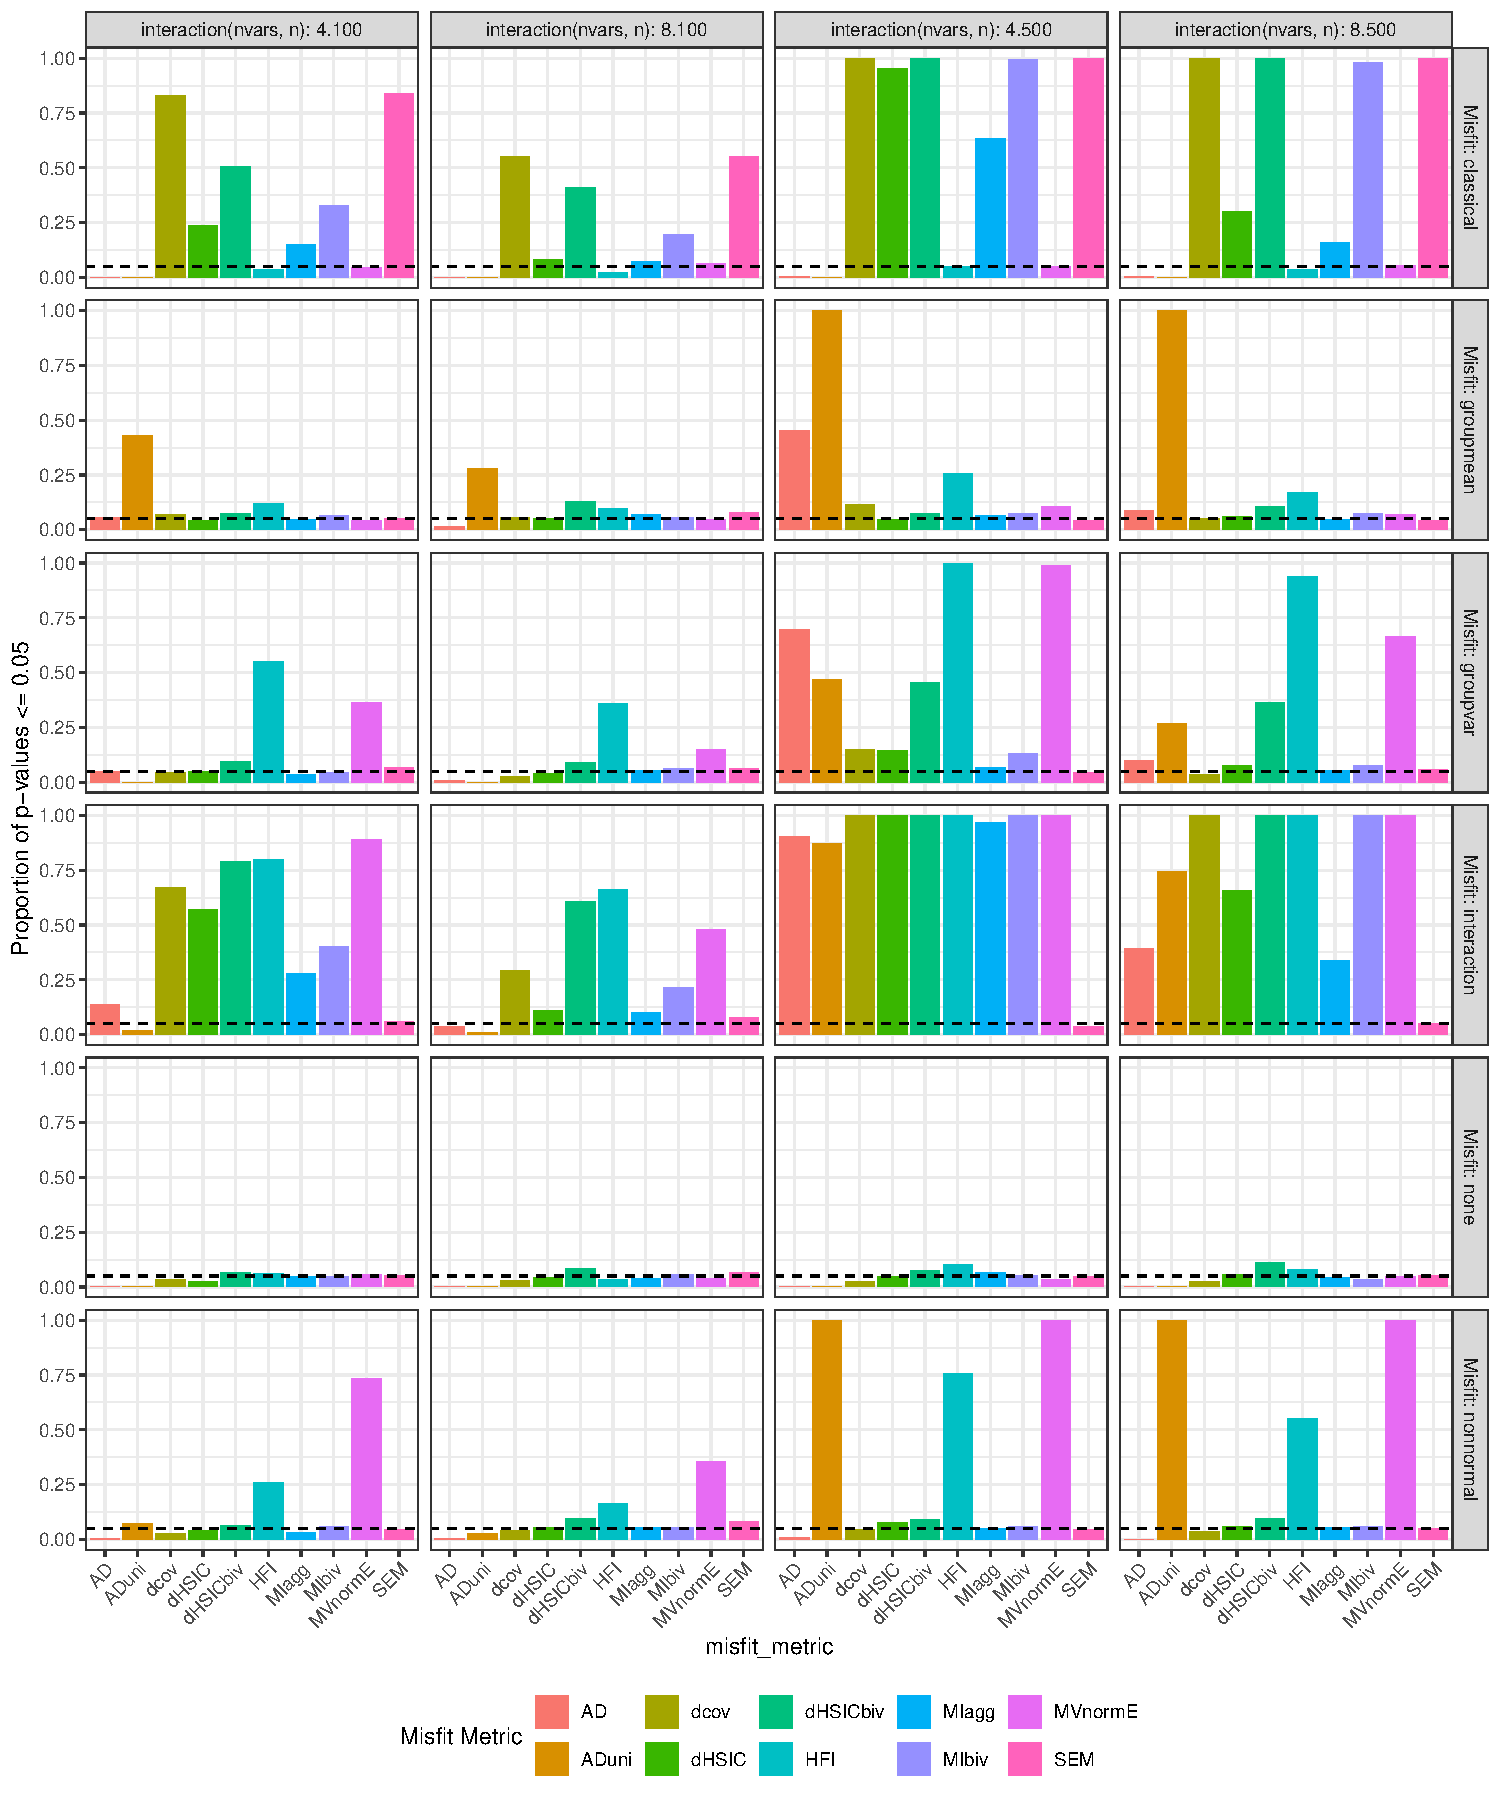
\includegraphics[width=.9\linewidth]{sim.pdf}
		\caption{Illustrative Detection Rates of Diagnostics Under Different Conditions}
		\label{fig:misfit_rates}
	\end{figure*}
	
	
	\begin{table*}[!htb]
		\caption{Illustrative Detection Rates in the SEM Misfit Simulation}
		\label{tab:sem_misfit_summary}
		\resizebox{\ifdim\width>\linewidth\linewidth\else\width\fi}{!}{
			\input{simtable}   
		}
	\end{table*}
	
	Figure~\ref{fig:misfit_rates} and Table~\ref{tab:sem_misfit_summary} summarize the proportion of $p \leq .05$ results across 500 replications per cell. The no-misfit results were generally reassuring. The energy test rejected in 3.6--5.6\% of replications and global dHSIC in 2.4--5.4\%, both close to the nominal .05 rate. Row-distance Anderson--Darling, marginal Anderson--Darling, and the Bonferroni-adjusted pairwise dCov screen were conservative, with rejection rates of 0--0.4\%, 0\%, and 0--2.2\%, respectively. The SEM comparator rejected in 5.0--8.6\% of replications, with the highest rate in the $n=100$, eight-variable cell. Overall, null behavior was good for an illustrative simulation, although the conservative diagnostics and one elevated SEM cell show that calibration should still be studied more systematically.
	
	The SEM chi-square test behaved primarily as a moment-fit comparator. It detected the omitted-covariance condition in 54.0--100\% of replications, with rejection increasing at $n=500$, but remained near its no-misfit behavior under the nonlinear, distributional, and subgroup conditions. Conversely, the energy test rejected in only 5.6--6.6\% of omitted-covariance replications despite the strong SEM signal. This contrast reflects the different targets of the diagnostics rather than a general ranking of their performance.
	
	The residual-distribution diagnostics responded differently across departures. The energy test showed broad sensitivity to omitted interactions, nonlinear curves, skewed marginals, heavy tails, and group-variance heterogeneity, particularly at $n=500$. At $n=500$, marginal Anderson--Darling checks rejected in 86.8--100\% of nonlinear-curve, skewed-marginal, and heavy-tail replications, but remained at or below 1.6\% for omitted interactions and group-variance heterogeneity. Row-distance Anderson--Darling checks were most responsive to nonlinear curves, omitted interactions, heavy tails, and group variance, with consistently weaker rejection in the eight-variable cells. The group-mean condition was a genuine mixture departure rather than a negative control, but it produced only modest signals: energy rejection reached 11.4\% and dHSIC rejection 10.0\% in the most responsive cell.
	
	Global dHSIC was sensitive to omitted interactions and nonlinear curves, especially with four variables and at $n=500$. In contrast, it remained near nominal for the skewed-marginal condition (3.8--6.6\%) and heavy tails (4.4--5.4\%), making these clearer negative controls for residual-dependence testing. It also reacted to the omitted covariance when the incorrect covariance left dependence after whitening, more strongly in the four-variable cells than with eight variables.
	
	The pairwise dCov results require a separate computational caveat. The reported statistic is the Bonferroni-adjusted minimum across all pairwise tests, not a measure of which pair was localized. With 199 permutations, the smallest attainable raw $p$-value is .005. After Bonferroni adjustment, the smallest attainable value is .030 for the six pairs in the four-variable condition but .140 for the 28 pairs in the eight-variable condition. Rejection at .05 was therefore impossible in every eight-variable cell, so the observed zeros are a permutation-resolution artifact and cannot support comparisons of sensitivity across dimensionality. In the four-variable cells, the screen frequently rejected for omitted covariance and nonlinear curves. A future run retaining this adjustment would need at least 559 permutations for rejection to be attainable with 28 pairs, with 999 or more preferable in practice. More generally, a larger simulation with refit-bootstrap calibration is still needed before making comparative performance claims \citep{bollen1992bootstrapping,pfister2018kernelbased}.
	
	\section{Empirical Example - Wage Data}
	
	\subsection{Prototype Software Implementation and Workflow}
	The empirical analysis uses the prototype implementation accompanying this paper rather than a released package. Its reader layer converts either a generic expectation list, a single-group \texttt{lavaan} fit, or a supported OpenMx model into a common \texttt{sem\_expectation} object containing the observed data, model-implied observed mean vector and covariance matrix, variable labels, and available SEM fit measures. One shared diagnostic engine then computes raw observation-level deviations, symmetric/ZCA residual coordinates for global diagnostics, variable-labelled conditional residuals, and rowwise squared Mahalanobis distances. The object reports exactly three targets: mean/covariance fit, full Gaussian observed-data fit, and conditional adequacy for a named variable. Cholesky innovations are retained only as an order-dependent comparison representation, without original-variable pair labels.
	
	The current implementation is deliberately narrow: continuous observed variables, one group, complete or listwise-complete data, and a model-implied mean and covariance interface. Permutation calibration is used for dHSIC and distance-covariance dependence tests; directional conditional tests are reported separately from transformed-coordinate screens. The current distribution and row-distance reference tests do not refit the SEM, and a requested parametric bootstrap is explicitly marked as not implemented. These limitations are reported in the object rather than hidden behind a single omnibus label. The core empirical workflow is executable as follows:
	
\noindent\begin{minipage}{\columnwidth}
\small
\begin{verbatim}
source("sem_misfit_api_prototype.R")
fit <- lavaan::sem(model, data = wage_core,
  meanstructure = TRUE, fixed.x = FALSE)
diagnostics <- sem_misfit(
  fit,
  calibration = "permutation",
  B = 999,
  adjust = "holm",
  seed = 70713)
as.data.frame(diagnostics)
sem_misfit_pairs(diagnostics)
sem_misfit_conditional_variables(diagnostics)
sem_misfit_variables(diagnostics)
plot(diagnostics, type = "pairwise_heatmap")
plot(
  diagnostics,
  type = "conditional_residual",
  variable = "logwage",
  against = "age_decade")
\end{verbatim}
\end{minipage}
	
	\subsection{Diagnostic Model, Classification, and Localization}
	The Wage data distributed with \citet{james2021introduction} contain 3000 observations on wages and worker characteristics from the Current Population Survey. We first fitted a deliberately conventional joint observed-variable path model in which log wage was regressed linearly on age and survey year, with age and year freely covarying:
	
	$$
	\text{log wage} \sim \text{age} + \text{year}.
	$$
	
	For the three observed variables, this model has no degrees of freedom for testing mean or covariance misfit. Classical SEM fit was therefore perfect by construction ($df = 0$, CFI $= 1.00$, RMSEA $= 0.00$, SRMR $< .001$). This first stage evaluates the joint mean and covariance structure; it is intentionally different from the covariate-conditional models used in the follow-up below.
	
	The previously generated analysis rejected mutual independence among its whitened residual coordinates (permutation dHSIC $p = .001$). Under the revised representation, such a result is reported as a probe against full Gaussian observed-data fit. The retained pairwise graphic ranks symmetric/ZCA coordinate pairs only; current substantive localization instead uses named conditional-residual tests and plots. The joint distribution, row-distance, and marginal residual checks also rejected their respective Gaussian references. The example therefore contains both broad distributional misfit and residual-coordinate dependence; it is not a pure nonlinear-dependence case.
	
	\begin{figure*}[!tbp]
		\centering
		\begin{minipage}{.49\linewidth}
			\centering
			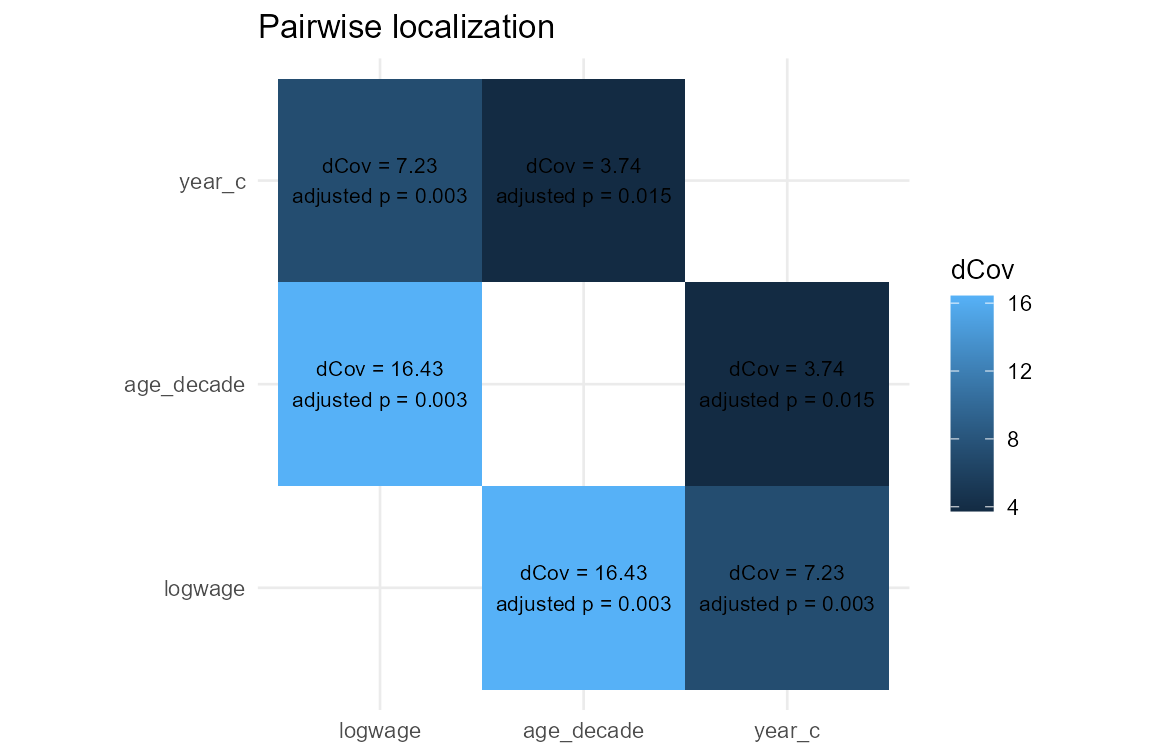
\includegraphics[width=\linewidth]{empirical_example_figures/wage_pairwise_heatmap.png}
		\end{minipage}
		\begin{minipage}{.49\linewidth}
			\centering
			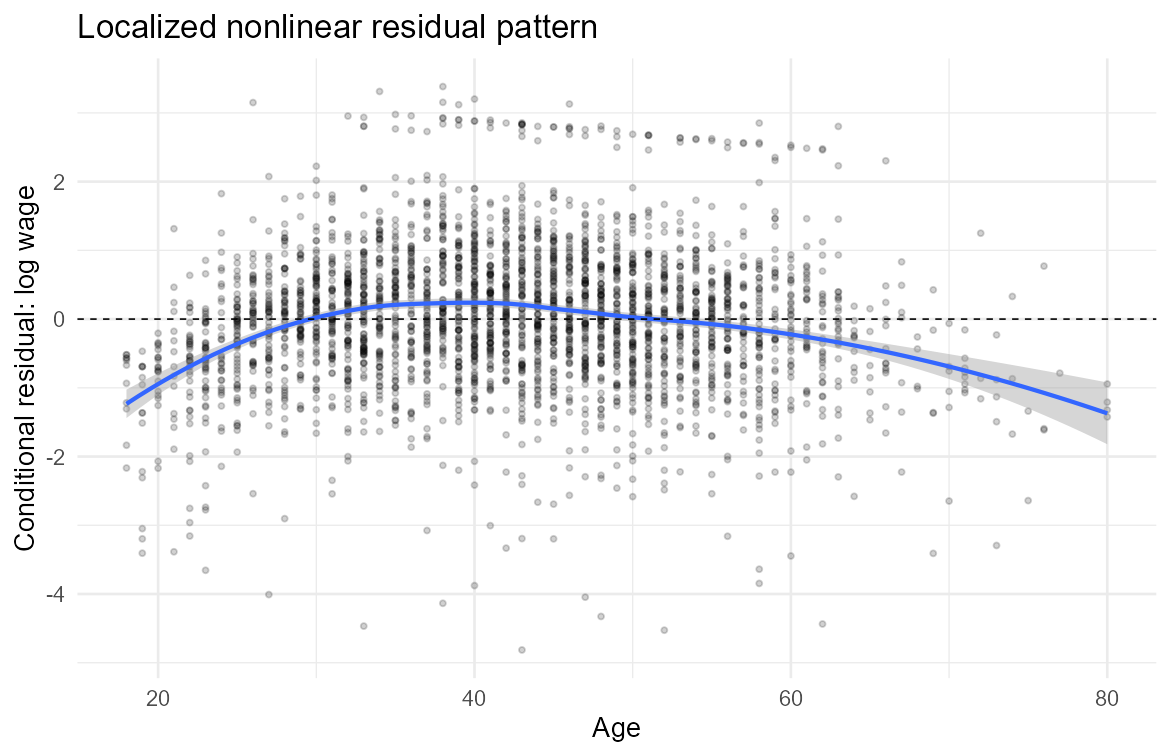
\includegraphics[width=\linewidth]{empirical_example_figures/wage_conditional_residual_by_age.png}
		\end{minipage}
		\caption{Software-Guided Localization in the Wage Example. The left panel is a retained illustrative pairwise-coordinate plot; under the revised prototype, its axes are symmetric/ZCA coordinates and are not original-variable residual labels. The right panel is generated from variable-labelled conditional residuals and shows the curved log-wage residual pattern over age.}
		\label{fig:wage_example}
	\end{figure*}
	
	Figure~\ref{fig:wage_example} makes the transition from diagnosis to model modification explicit. The heatmap is retained transformed-coordinate exploration and does not translate a coordinate pair into an original-variable claim. The separately variable-labelled conditional plot shows log wages underpredicted around midlife and overpredicted at younger and older ages, suggesting that the conditional mean is inadequate; this plot alone does not rule out scale or broader conditional-distribution explanations.
	
	\subsection{SEM Modification and Spline Sensitivity Check}
	We next fitted two matched covariate-conditional path models in \texttt{lavaan}. Both included centered age, centered age squared, and survey year as fixed predictors of log wage. In the linear model, the age-squared path was fixed to zero; in the quadratic model, it was freely estimated. Keeping the same observed variables in both fits yields a valid one-degree-of-freedom nested comparison. Freeing the quadratic path improved fit, $\Delta\chi^2(1) = 196.94$, $p < .001$, and reduced AIC from 2091.19 to 1896.25. The quadratic coefficient was negative ($b = -0.000524$, $SE = 0.000037$), matching the rise and later decline visible in Figure~\ref{fig:wage_example}.
	
	The age--outcome-residual distance correlation fell from .129 in the linear conditional SEM to .063 in the quadratic SEM. It remained detectable ($p = .001$), so the polynomial should be described as a substantial but incomplete modification rather than a repaired model. As a sensitivity check, an \texttt{mgcv} smooth gave an effective degrees of freedom of 4.60 ($p < .001$) and reduced the distance correlation further to .048 ($p = .022$). The spline therefore supports the qualitative conclusion that the age pattern is curved, but it is not the primary workflow or evidence that the residual structure has been fully explained.
	
	The diagnostic and modification stages have different targets. The initial \texttt{sem\_misfit()} call evaluates a joint mean/covariance model. The follow-up evaluates a nonlinear conditional mean for log wage. We do not rerun the joint diagnostics as if the polynomial or spline were represented by the current expectation interface, which does not yet accept case-specific conditional means. Extending that interface is future software work.
	
	Although Wage contains one endogenous variable, the observed-basis modification is not intrinsically univariate. In a multivariate path system the same centered basis terms can enter several equations while residual relations among outcomes remain part of the SEM, for example:
	
\begin{verbatim}
outcome1 ~ age_c + age_c2 + x
outcome2 ~ age_c + age_c2 + x
outcome1 ~~ outcome2
\end{verbatim}
	
	Thus the empirical dataset demonstrates one equation, whereas the SEM modification generalizes directly to multiple endogenous outcomes. We did not use an SEM tree because the observed residual pattern is smooth rather than evidence for discrete moderator-defined subgroups; recursive partitioning would answer a different heterogeneity question and approximate the age curve with thresholds.
	
	The example remains descriptive. It does not establish a causal age effect, identify a uniquely correct wage model, or imply that residual diagnostics select revisions automatically. It demonstrates a reproducible SEM workflow in which standard moment fit, software-based residual classification, substantive localization, and an explicitly evaluated model modification remain separate steps.
	
	
	\section{Nonlinear Misspecification Found -- What Now?}
	
	A residual diagnostic is not a model-repair algorithm. A significant residual-distribution or residual-dependence test says that a specific residual null is implausible; it does not say which parameter should be freed, which nonlinear term should be added, or whether the resulting model would have better external validity. The practical task is therefore to move from detection to classification, localization, and theory-guided follow-up while keeping the diagnostic and modeling stages conceptually separate.
	
	\subsection{Detect and Name the Failed Residual Null}
	The first step is to record which diagnostic rejected and what null hypothesis that diagnostic targeted. A poor standard SEM chi-square or residual covariance pattern points to mean or covariance misfit, the usual target of SEM model fit. A global energy-distance or row-distance diagnostic points to a broad violation of the fitted Gaussian residual distribution \citep{rizzo2016energy}. Marginal residual-normality checks point to variable- or coordinate-specific skewness, heavy tails, or outliers. A dHSIC, distance-covariance, or related independence diagnostic points instead to residual dependence after whitening \citep{pfister2018kernelbased,karch2024pearsons}. Heteroscedasticity summaries, rowwise distances, or moderator-specific residual-scale checks point to cases or regions where the residual variance changes. These signals can co-occur, but they should be reported as different forms of evidence rather than collapsed into a generic claim of nonlinear misspecification.
	
	\subsection{Classify the Diagnostic Signal}
	After detection, the signal should be classified before any model is changed. A useful classification separates at least five possibilities. First, mean or covariance misfit suggests that the linear SEM structure itself may be wrong. Second, marginal distributional misfit suggests variable-specific transformations, heavy tails, outliers, floor or ceiling effects, or other distributional features that may not imply residual dependence. Third, joint distributional misfit suggests that the full residual cloud differs from the fitted Gaussian reference, possibly because of tails, mixtures, outliers, dependence, or heterogeneity. Fourth, residual-dependence misfit suggests that the fitted mean and covariance structure has not removed higher-order association among residual coordinates. Fifth, heterogeneity signals suggest that parameters, residual scales, or case distances may vary over observed covariates, fitted values, or latent subgroups. This classification prevents a common overinterpretation: a nonnormal residual distribution is not automatically evidence for an omitted interaction, and an independence-test rejection is not automatically evidence for a particular structural path.
	
	\subsection{Localize Before Revising}
	Localization should identify where follow-up modeling is worth the cost. Pairwise residual-dependence heatmaps can rank residual-coordinate pairs for distance covariance, HSIC, or dHSIC-style statistics. Variable-wise marginal checks can show whether a global distributional signal is concentrated in one indicator or spread across the measurement battery. Rowwise squared residual distances can identify outlying cases or potential subgroups, but these distances should be interpreted as case-level extremeness rather than as proof of a specific nonlinear mechanism. Conditional residual plots are useful when whitened residual coordinates are hard to label substantively: plotting a variable-labeled conditional residual against fitted values, observed covariates, time, or theoretically plausible moderators can reveal curvature, changing variance, or subgroup separation. Moderator scans and residual-scale plots should be treated as exploratory unless the moderator and test were specified in advance, and pairwise/local tests require multiplicity control or clear ranking language.
	
	\subsection{Choose Follow-Up Models That Match the Signal}
	Model follow-up should be tied to the diagnostic pattern. If classical SEM fit or residual covariance diagnostics fail, the natural first candidates are ordinary SEM revisions: omitted paths, cross-loadings, correlated residuals, or revised measurement structure, constrained by substantive theory. If marginal residual distributions drive the signal, follow-up may involve transformations, robust or heavy-tailed distributional assumptions, explicit outlier modeling, or sensitivity analyses that compare conclusions with and without influential observations \citep{satorra1994corrections,jia2026obtaining}. If pairwise or joint residual-dependence diagnostics indicate higher-order association, theory-guided nonlinear paths, latent interactions, product terms, or spline terms are more directly matched to the signal than generic model modification \citep{mcdonald1962general,klein2000maximum,irmer2024estimating,cox2025comparing}. If residual patterns vary with an observed covariate, moderated SEM, local structural equation modeling, or other smooth moderator-specific approaches can estimate how parameters change across that covariate \citep{briley2015nonparametric}. If rowwise distances, residual scales, or heatmaps suggest discrete subgroups, mixture models, latent classes, structural equation model trees, or SEM forests provide more direct follow-up tools than a single pooled SEM \citep{lubke2005investigating,brandmaier2013structural,arnold2021score,silvaDiaz2025evaluation}. Bayesian SEM, Bayesian fit indices, and posterior predictive checking can also be useful when the follow-up question concerns approximate restrictions, uncertainty in complex models, or sensitivity to prior assumptions \citep{muthen2012bayesian,garnierVillarreal2020adapting}.
	
	\subsection{Report Diagnostics as Sensitivity Evidence}
	The final step is transparent reporting. Researchers should state which residual representation was used, which diagnostics were run, how p-values or reference distributions were calibrated, and whether local analyses were planned or exploratory. Follow-up models should be described as theoretically motivated responses to a diagnostic signal, not as automatic repairs discovered by the diagnostics. If several candidate revisions are explored, the manuscript should distinguish confirmatory tests from exploratory triage and should report whether the original substantive conclusions are robust across reasonable alternatives. In this role, residual diagnostics function as sensitivity checks and guides for model development: they can show that the fitted SEM leaves important structure in the data, but they cannot by themselves prove that a particular alternative model is the correct explanation.
	
	
	\section{Conclusion}
	
	The simulation study underscores the limits of traditional SEM chi-square tests for detecting residual structure that does not substantially alter mean and covariance fit, including interaction terms in the present setup. In contrast, residual-based diagnostics can be selected for different diagnostic targets. Energy and row-distance distribution checks showed broad sensitivity to departures from the fitted Gaussian residual reference, but this sensitivity also includes univariate nonnormality, heavy tails, and subgroup heterogeneity, and should not be interpreted as specific evidence of nonlinear dependence. Permutation-calibrated dHSIC instead targeted residual dependence after whitening. Individual pairwise distance-covariance tests can support localization, but the aggregate pairwise screen reported in the simulation was constrained by permutation resolution after multiplicity adjustment, particularly in the eight-variable conditions.
	
	Several limitations define the intended scope of these results. No-misfit rejection rates were close to nominal for energy and dHSIC and conservative for the other residual diagnostics, but the simulations remain illustrative rather than a complete validation study. Stronger calibration work is still needed, especially refit-bootstrap calibration that accounts for fitted-parameter uncertainty. The empirical example is an observed-variable path model, not a latent-variable measurement example, and its residual diagnostics show both distributional and dependence signals. It demonstrates the prototype workflow end to end for a \texttt{lavaan} fit, including tabular and graphical localization, but the nonlinear conditional follow-up is evaluated separately because case-specific conditional expectations are not yet part of the shared interface. The software contribution is therefore best understood as a prototype workflow for continuous, single-group, complete-data settings; broader SEM readers, categorical indicators, missing-data diagnostics, multigroup models, case-specific conditional expectations, and default bootstrap inference remain future package work.
	
	When residual diagnostics indicate additional structure, the next step should be classification and localization rather than automatic modification. Pairwise heatmaps, variable-wise residual checks, rowwise distances, moderator plots, and posterior predictive or bootstrap comparisons can guide follow-up models, but the follow-up should remain theory-guided and reported as sensitivity evidence unless it was specified and calibrated in advance. Used in this way, residual diagnostics extend SEM practice by making different forms of misfit visible while preserving the distinction between detecting a problem, locating its empirical pattern, and defending a substantive model revision.
	
	
	
	
	
	
	
	
	
	
	
	
	\printbibliography
\end{document}
